\chapter{Medical Imaging and Image Segmentation}
%

The first steps in image-based modeling and simulation involve image acquisition, image processing, and image segmentation. Several techniques are available to produce three-dimensional image data of an anatomical region of interest and are reviewed herein. State-of-the art image processing and image segmentation approaches are summarized in this section as well.

%%%%%%%%%%%%%%%%%%%%%%%%%%%%%%%%%%%%%%%%%%%%%%%
%%%%%%%%%%%%%%%%%%%%%%%%%%%%%%%%%%%%%%%%%%%%%%%
\section{Imaging Approaches}
\label{Imaging Approaches}

Medical imaging is the process of generating discrete image representations of biological tissues. Of the many imaging modalities found in clinical and research settings, the most prevalent are magnetic resonance imaging (MRI) and x-ray computed tomography (CT). Both approaches are \textit{tomographic} in that they produce a series of two-dimensional images representing thin slices through the region, that are subsequently combined to produce a three-dimensional volume representation \cite{larobina_murino_2014}. The data measured during acquisition are different for each modality, and thus the use case typically governs which technique is most appropriate. Several other imaging techniques exist - some of which provide more information than do MRI and CT - and are briefly presented in this section as well. Finally, typical data storage and file formats are discussed.

\subsection{Magnetic Resonance Imaging}
\label{Magnetic Resonance Imaging}

Magnetic resonance imaging (MRI) is the process of generating images via the physical phenomenon of nuclear magnetic resonance (NMR), in which nuclei in a magnetic field absorb and re-emit electromagnetic radiation at their \textit{resonant frequency}~\cite{NMR}. Gradients in the magnetic field are used to encode the response at different locations in the region. MRI provides excellent soft tissue contrast, for tissues such as gray and white matter in the brain, articular cartilage, bone marrow, muscle, and ligaments. Unlike CT, it does not use any harmful ionizing radiation~\cite{waldman_campbell}. A brief description of the basic physics in acquiring an MRI follows.

A strong external magnet generates a magnetic field $B_0\bm{e}_z$ that is constant in time and space, within which the patient or object is placed. For most clinical applications the strength of this field is 1.5 Tesla or 3 Tesla. The $z$ direction corresponds to the image slice direction. Shim coils are used to correct or "shim" the magnetic field so as to ensure good field homogeneity, leading to a quality received signal in generating the image~\cite{jacobs_2007}. Nuclear dipole moments in certain atoms align either in parallel or anti-parallel to the direction of the applied magnetic field, similarly to how a bar magnet orients itself in the presence of an external magnetic field~\cite{hendrick_1994}. The parallel orientation provides a slightly lower energy state than that for the anti-parallel orientation, and thus the dipole moments slightly prefer to align with the direction of the applied magnetic field. Prior to the external magnetic field, the random orientation of the nuclear magnetic dipoles in the tissue produce a zero net magnetization. Following the imposition of a static magnetic field, a net magnetization of tissue $M_0\bm{e}_z$ is produced from the preferential alignment of dipoles. See \figref{mr1}. Due to the prevalence of hydrogen in biological tissues, most notably in water and fat, MR imaging is typically based on the behavior of the nuclear magnetic dipole of hydrogen.
\begin{figure}[ht]
\centering
\subfigure[]{%
		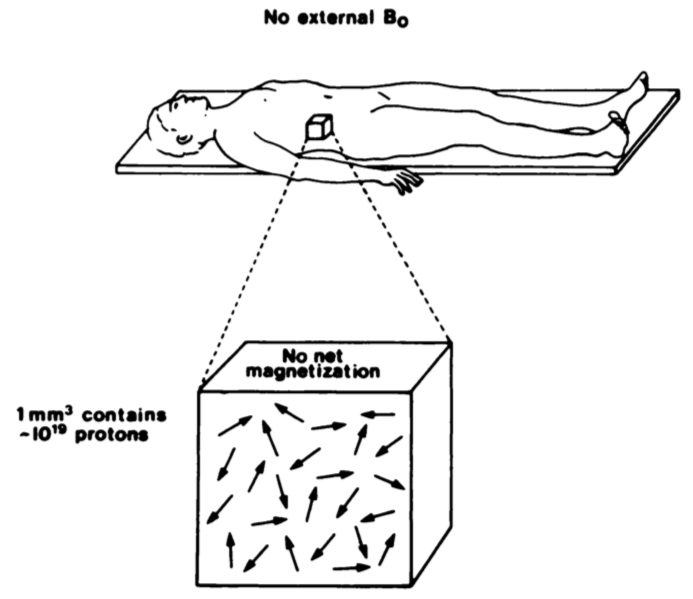
\includegraphics[scale=0.33]{media/0-imaging/mr1a.png}
\label{fig:mr11}}
\subfigure[]{%
		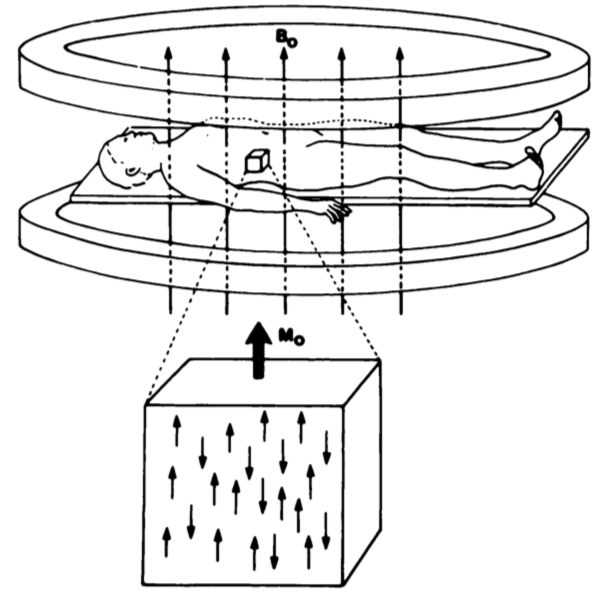
\includegraphics[scale=0.33]{media/0-imaging/mr1b.png}
\label{fig:mr12}}
%
\caption{Net magnetization $M_0$ in a voxel of tissue (a) prior to, and (b) following the application of a static external magnetic field $B_0$~\cite{hendrick_1994}}
\label{fig:mr1}
\end{figure}

If the net magnetization is perturbed from pointing in the same direction of a magnetic field $B\bm{e}_z$, the new magnetization $M$ \textit{precesses} about the $z$ axis. The \textit{precessional frequency} or {Larmor frequency} $\omega$ is defined by the following relationship:
\begin{equation}
\omega = \gamma B
\end{equation}

where the constant $\gamma$ is the \textit{gyromagnetic ratio}, which is 42.6 MHz/T for hydrogen. In MR imaging, the net magnetization is tipped away from the direction of $B_0$ by applying a radio-frequency (RF) pulse that oscillates exactly at the Larmor frequency. The precessing transverse magnetization produces a changing magnetic field, which induces an electric current that oscillates at the Larmor frequency and is recorded by the receiver coil. See \figref{mr2}.

\begin{figure}[ht]
\centering
\subfigure[]{%
		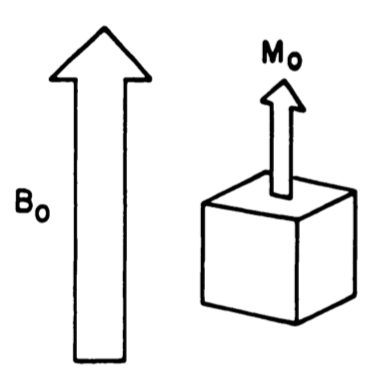
\includegraphics[scale=0.25]{media/0-imaging/mr2a.png}
\label{fig:mr21}}
\subfigure[]{%
		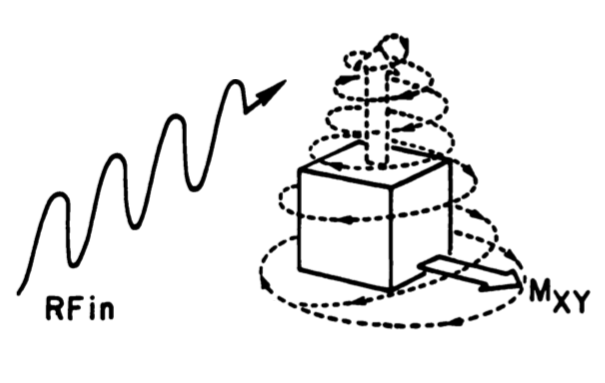
\includegraphics[scale=0.25]{media/0-imaging/mr2b.png}
\label{fig:mr22}}
\subfigure[]{%
		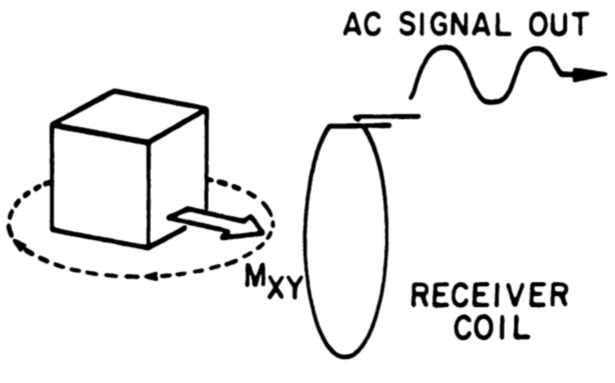
\includegraphics[scale=0.25]{media/0-imaging/mr2c.png}
\label{fig:mr23}}
%
\caption{Basic premise of MRI: (a) An external magnetic field $B_0$ causes net magnetization $M_0$ of the voxel of tissue, pointing in the same direction as the applied field, (b) RF pulse applied at the precessional frequency of hydrogen causes the magnetization vector to tilt from a longitudinal direction into the transverse plane, and (c) the amplitude, frequency, and phase of the time-varying signal from the transverse magnetization $M_xy$ is recorded~\cite{hendrick_1994}}
\label{fig:mr2}
\end{figure}

In order for the receiver coil to distinguish between different locations in the object, \textit{spatial localization} of the MR signal is achieved by applying linear magnetic field gradients in each of the three spatial directions. Namely, the new spatially varying magnetic field $B(\bm{x})\bm{e}_z$ (still pointing in $z$ direction), following the imposition of magnetic gradients, becomes:
\begin{equation}
B(\bm{x}) = B_0 + \bm{G}(t) \cdot \bm{x}
\label{eqn:gradient}
\end{equation}

The magnetic field gradient $\bm{G}(t) = (G_x, G_y, G_z)$ is applied in stages, to be discussed shortly. Multiplying \eqnref{gradient} by $\gamma$ yields:
\begin{equation}
\omega(\bm{x}) = \omega_0 + \bm{G}(t) \cdot \bm{x}
\label{eqn:freq}
\end{equation}
Thus, each RF signal oscillates at the appropriate frequency to excite and record information for each unique voxel in the image. Specifically, the magnetic gradient $G_z$ and corresponding RF pulse are first turned on to excite a particular slice (or section) of tissue. Excitation here refers to the perturbation of the net magnetization from the $z$ direction into the transverse plane. $G_z$ is referred to as the \textit{slice-selection gradient}. The resolution of the image in the $z$ direction may be increased by reducing the bandwidth of the RF pulse or increasing the strength of the applied gradient. To resolve the selected section into voxels, gradients are applied separately in each of the two in-plane directions $x$ and $y$. The magnetic gradient $G_y$ is applied and removed between the events of signal excitation and signal measurement. While turned on, it causes hydrogen nuclei located in a slightly stronger magnetic field to precess faster for a brief period of time. When the gradient is turned off, different strips maintain the same precessional frequency within the same slice, but a fixed phase difference now exists among them. $G_y$ is referred to as the \textit{phase-encoding gradient}. Finally, the magnetic gradient $G_x$ alters the resonant frequency along the $x$ direction. It separates each strip into voxels, each voxel resonating at a different frequency. $G_x$ is applied at the time of signal measurement and is referred to as the  \textit{frequency-encoding gradient} or the {readout gradient}. The resolution of the in-plane image may be increased by increasing the number of pulse sequence acquisitions and subsequent measurements. See Figure \figref{mr3} for a visual representation.

\begin{figure}[ht]
\centering
\subfigure[]{%
		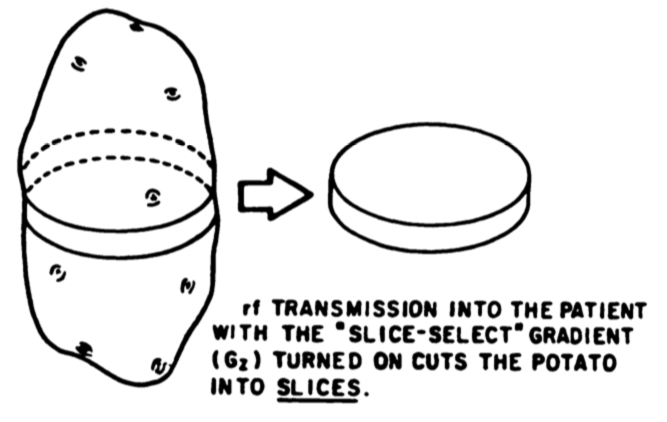
\includegraphics[scale=0.21]{media/0-imaging/mr3a.png}
\label{fig:mr31}}
\subfigure[]{%
		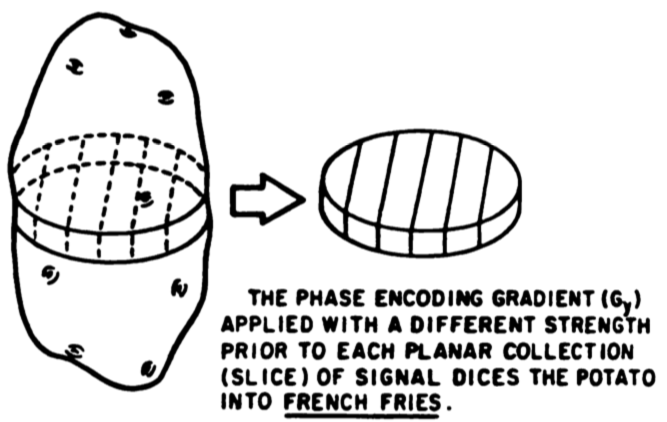
\includegraphics[scale=0.21]{media/0-imaging/mr3b.png}
\label{fig:mr32}}
\subfigure[]{%
		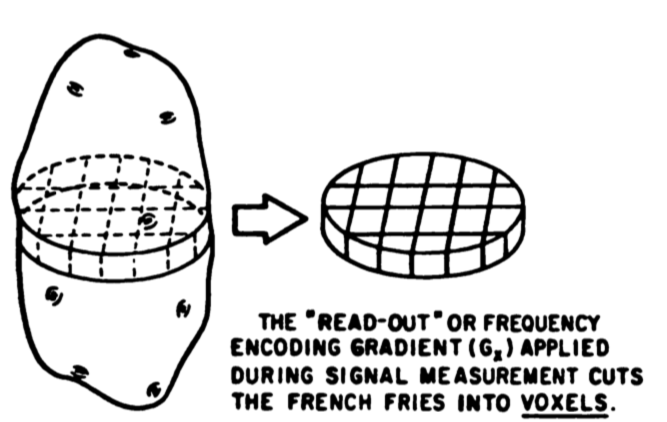
\includegraphics[scale=0.21]{media/0-imaging/mr3c.png}
\label{fig:mr33}}
%
\caption{Visual representation of the process of spatial localization based on successful application of magnetic gradients: (a) slice-selection gradient, (b) phase-encoding gradient, and (c) frequency-encoding gradient~\cite{hendrick_1994}}
\label{fig:mr3}
\end{figure}

MRI signal intensity at a particular voxel typically depends on the proton density of the tissue (via the strength of the net magnetization $M_0$) and two relaxation times T1 and T2 as the perturbed net magnetization exponentially decays to its original state following an RF pulse. Following a typical $90^{\circ}$ RF pulse, which maximizes the transverse magnetization $M_{xy}$, the relaxation times are defined as such:
\begin{equation}
M(t) = M_0(1 - e^{(-t/T1)})
\end{equation}
\begin{equation}
M_{xy}(t) = M_{xy}e^{(-t/T2)}
\end{equation}
Namely, \textit{spin-lattice}, \textit{longitudinal}, or \textit{T1 recovery time} corresponds to the recovery of the longitudinal magnetization $M_0$. This reorientation is caused by the transfer of energy from the excited magnetic dipoles to the surrounding lattice of molecules. The \textit{transverse}, \textit{spin-spin}, or \textit{T2 recovery time} corresponds to the dephasing of magnetic dipoles as they precess. This dephasing is caused by different magnetic environments for different hydrogen nuclei within the same voxel as the transverse magnetization decays.

Tissue contrasts are created based on the strength and timing of the RF pulse; this is known as the \textit{MR sequence}. The parameters in MR pulse sequences weight the influence of proton density, T1, and T2 differently in the final MR signal. The most basic MR sequences include: Proton Density (PD), T1-weighted (T1W), and T2-weighted (T2W), each of which provide different tissue contrasts. The choice of an MR sequence will depend on the tissues and applications of interest of the scan. A number of references are available  \cite{nishimura_2010, brown_semelka_2003, webb_2003} for a more detailed description of T1, T2, the parameters of an MR sequence, and their relationship in creating tissue contrast.

For each voxel in a slice, the amplitude, phase, and frequency of the time-varying MR signal is recorded by the receiver coil in the \textit{frequency domain}, or what is known as \textit{k-space}. For each slice, the frequency domain is converted to the spatial domain (i.e., the two-dimensional image for a particular slice) via 2D inverse Fourier transform. K-space can be used to identify artifacts, remove noise, and enhance contrast~\cite{imaios}. Please refer to the references in this section for more detail on k-space and its manipulations. Finally, each 2D image is combined to form a 3D grayscale image corresponding to the object scanned. The intensity at each voxel in the three-dimensional rectilinear grid is a weighted proton density.

\subsection{X-Ray Computed Tomography}
\label{X-Ray Computed Tomography}

houndsfield units

\subsection{Additional Imaging Modalities}
\label{Other Imaging Modalities}

\subsection{File Formats}
\label{Data Format-IMG}

Medical images are typically stored as a combination of a short \textit{header} followed by \textit{pixel data}. The header is typically stored in ASCII format and the pixel data is typically binary. They may be found in the same file or in separate ones. Pixel data is often stored either as a set of two-dimensional images representing each slice, or as a single block of information corresponding to the 3D volume. In either case, data is stored as a 1D array, from which the data can be unrolled based on the axis ordering specified in the header. The header provides metadata to allow software to read and store the image based on the pixel data. Namely, the header contains the matrix dimensions, image resolution, image origin, axis order, data type of the pixel data (i.e., unsigned char, int, etc.), endianness of the pixel data, and data compression encoding (e.g., raw, gzip, bzip2). Additional information may be provided as well, including patient data, image acquisition parameters (e.g., MRI pulse sequence), and date of acquisition. On the clinical side, DICOM (Digital Imaging and Communications in Medicine) files are by far the most popular format for storing medical images, due to it's extensive metadata including patient information and image acquisition protocol. On the research side, several formats are available, including MATLAB~\cite{MATLAB}, NRRD (Nearly Raw Raster Data)~\cite{nrrd}, NIfTI (Neuroimaging Informatics Technology Initiative)~\cite{nifti}, and Analyze~\cite{analyzedirect}. These file formats are different flavors of the general format described above. They are geared more towards image post-processing compared to DICOM, by way of less detailed metadata sections.


%%%%%%%%%%%%%%%%%%%%%%%%%%%%%%%%%%%%%%%%%%%%%%%
%%%%%%%%%%%%%%%%%%%%%%%%%%%%%%%%%%%%%%%%%%%%%%%
\section{Image Segmentation Approaches}
\label{Image Segmentation Approaches}

Arguably the most challenging task in the workflow is the subsequent image processing and \textit{segmenting} of the image of interest.

\begin{figure}[ht]
\centering
\subfigure[]{%
		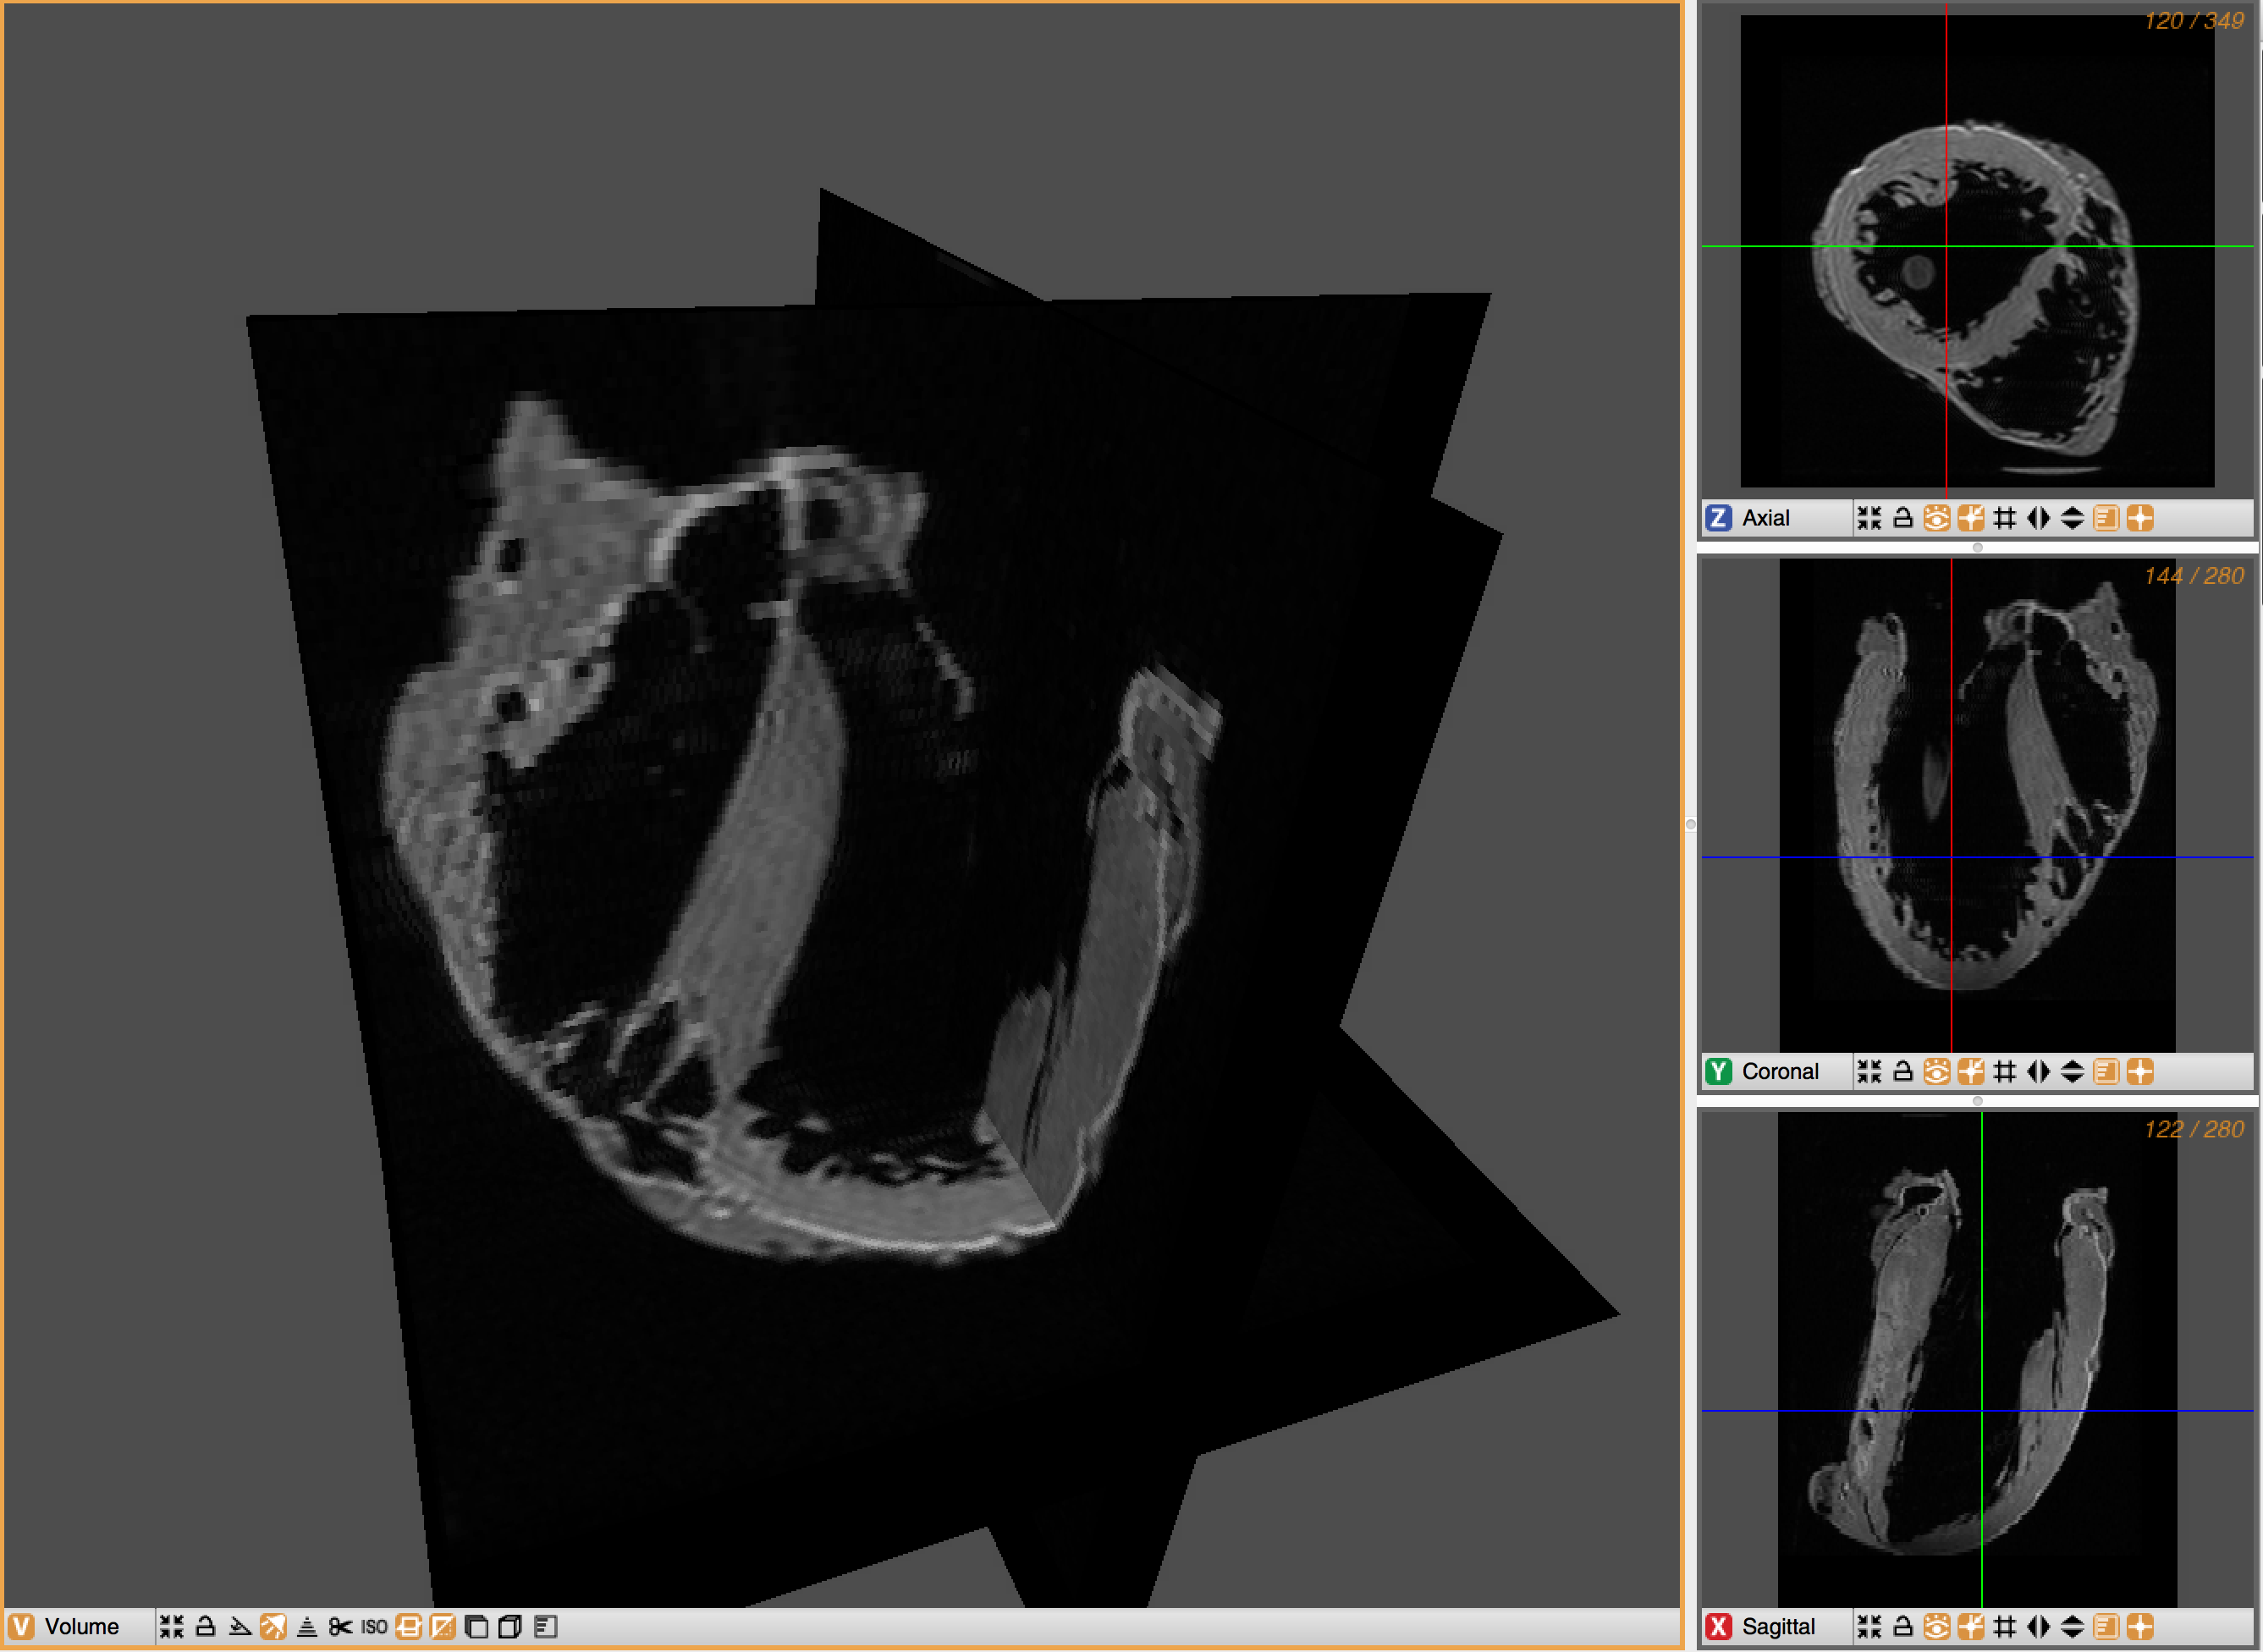
\includegraphics[scale=0.165]{media/1-seg3d/1-raw.png}
\label{fig:seg1}}
\subfigure[]{%
		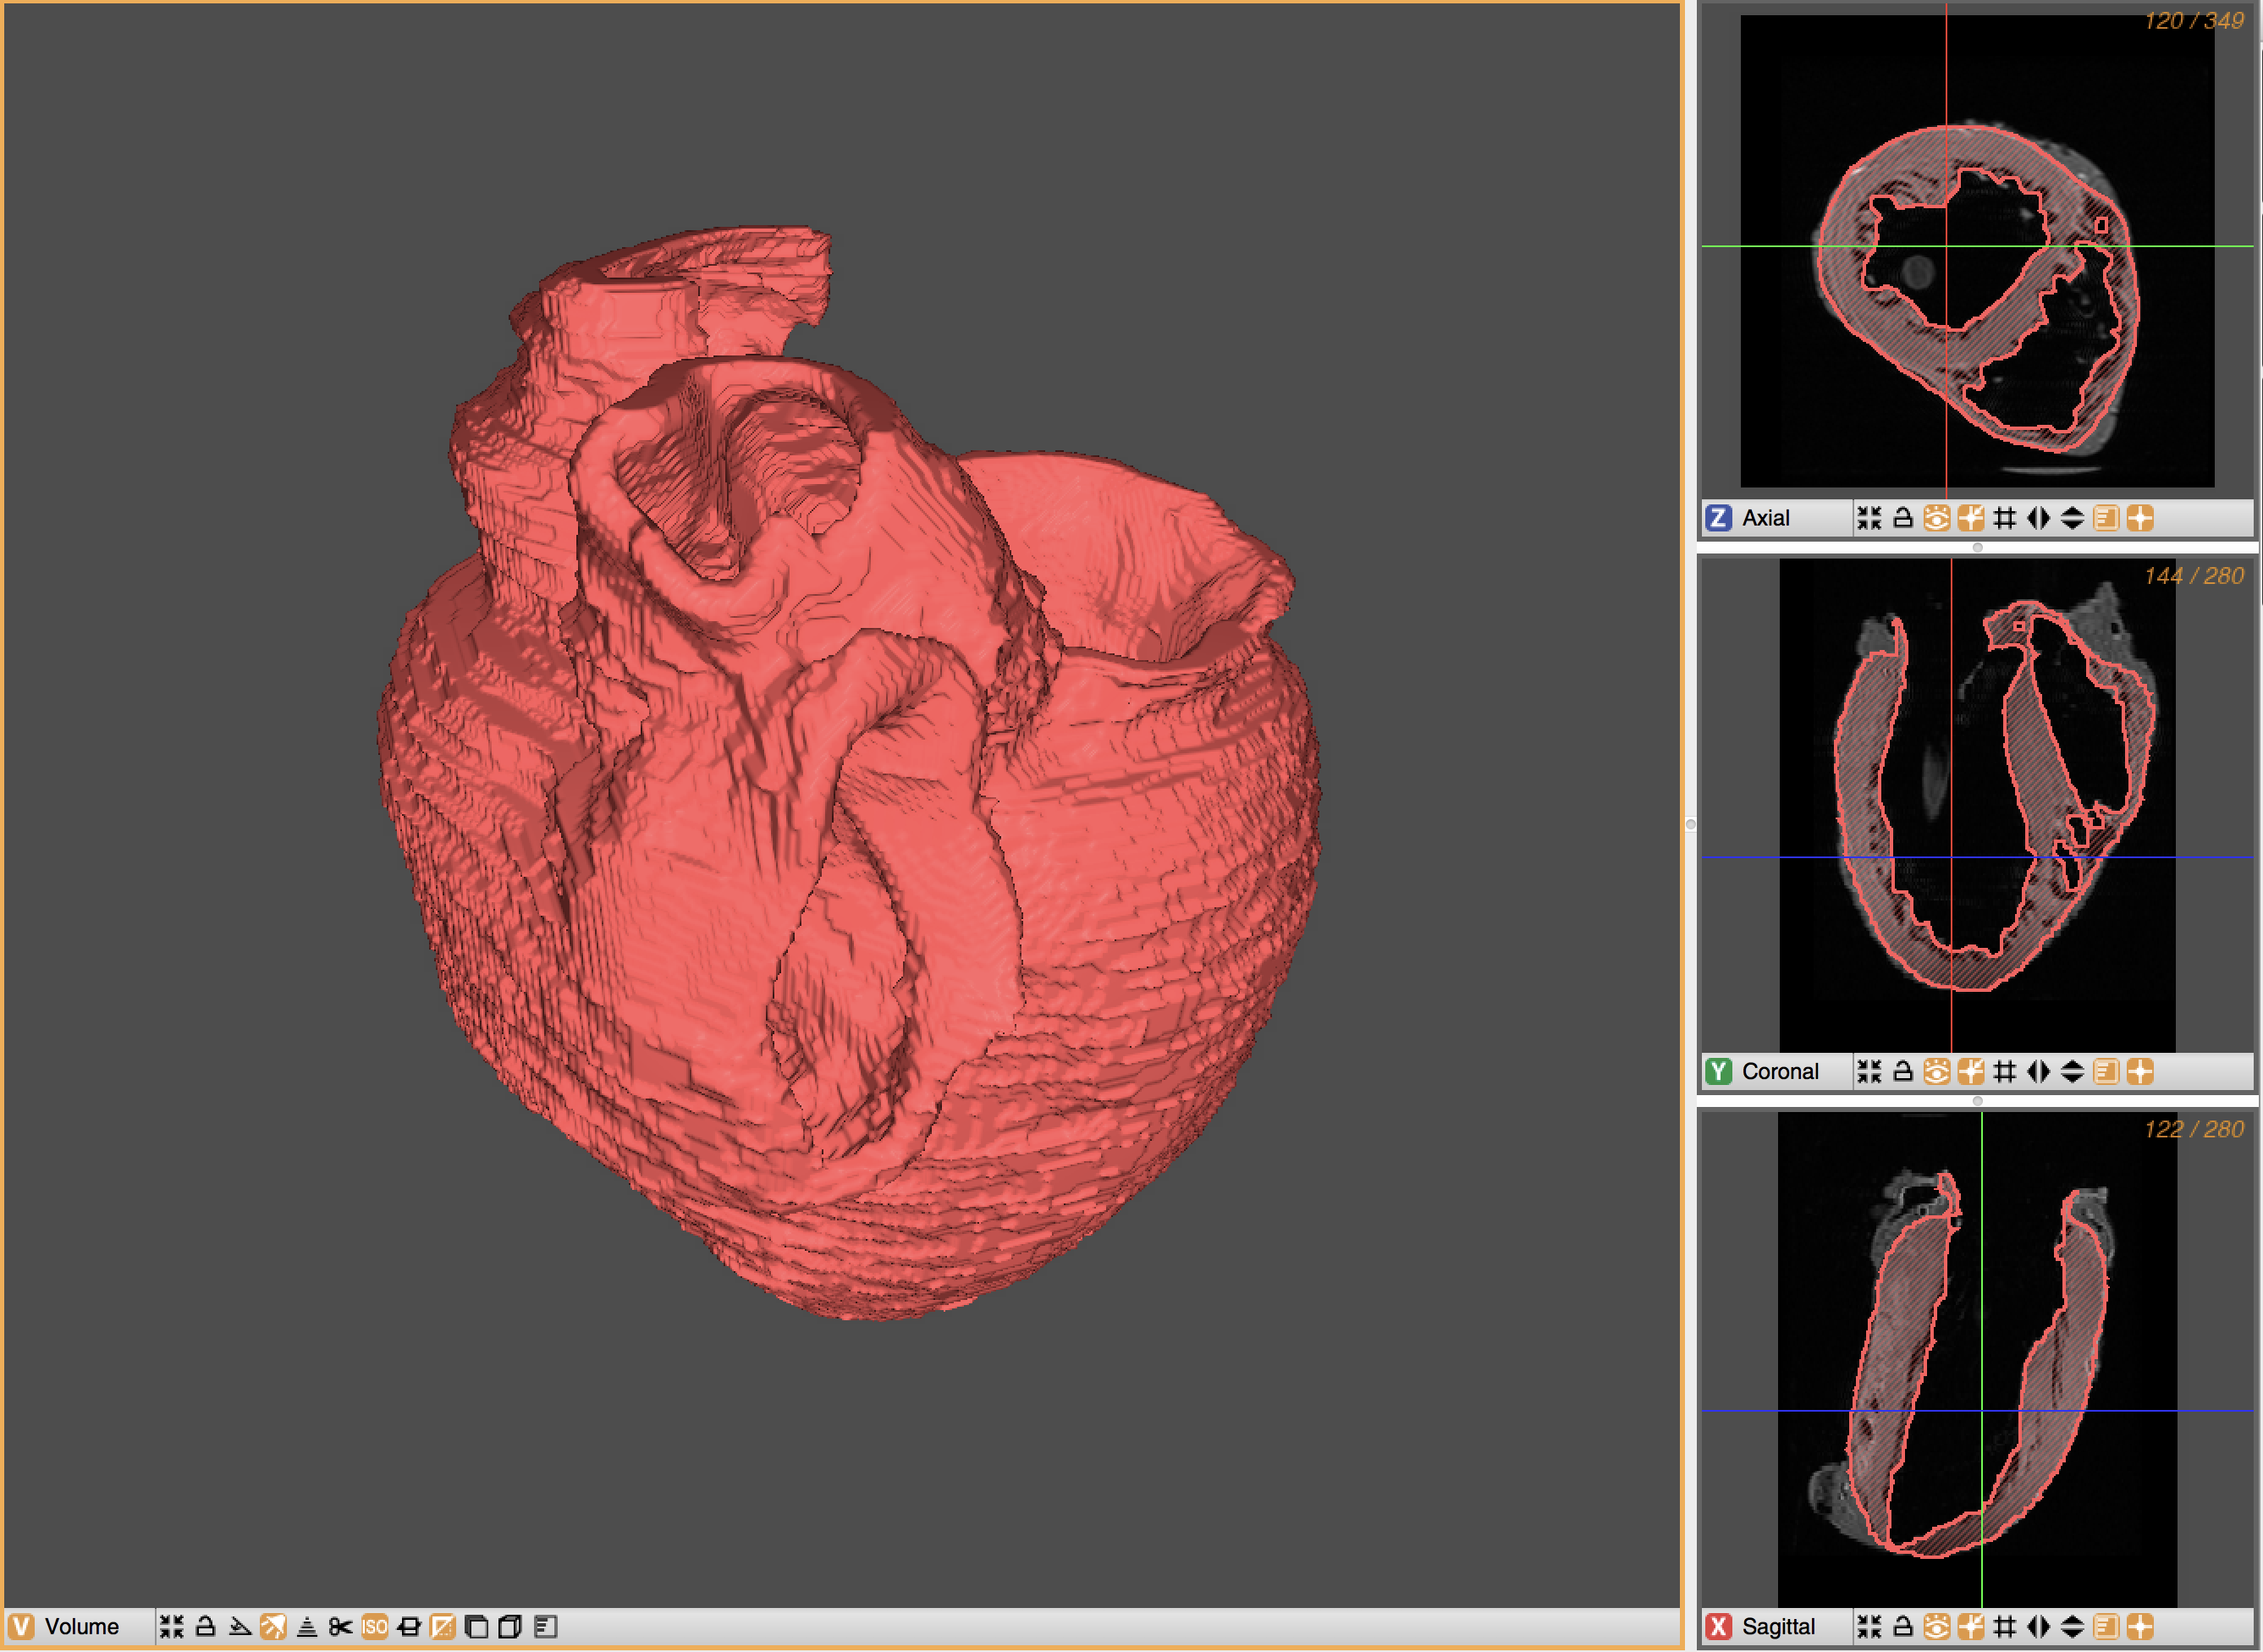
\includegraphics[scale=0.165]{media/1-seg3d/2-seg.png}
\label{fig:seg2}}
%
\caption{(a) MRI of \textit{ex-vivo} human heart, and (b) resulting segmented image mask}
\label{fig:seg}
\end{figure}

Talk about image processing/filtering here. Gaussian blur, mean filter, median filter.
Intravenous or intra-articular contrast agents may be administered to the patient to further enhance contrast in the original image. Image segmentation techniques may well take advantage of the image modality and image acquisition parameters. 

\subsection{Thresholding Methods}
\label{Thresholding Methods}

\subsection{Region-Growing Methods}
\label{Region-Growing Methods}

\subsection{Neural Networks}
\label{Neural Networks}

\subsection{Manual Methods}
\label{Manual Methods}

\subsection{File Formats}
\label{Data Format-SEG}
